\section{Ergebnisse und Diskussion}
\label{sec:discuss}

\subsection{Modellwahl}
\label{ssec:discuss:modelselect}
Unter Anwendung der in Abschnitt \ref{ssec:modellselektion} bzw \ref{ssec:impl:modelwahl} vorgestellten Methode wurde aus einem 149 Prädiktoren umfassenden Maximalmodell das in Tabelle \ref{table:model_parameters} angegebene, 50 Prädiktoren große Modell anhand des kleinsten $C_p$-Wertes von $\m{\approx3.92}$ als optimales Modell ausgewählt.\\
\begin{figure*}[ht]
    \centering
    \begin{tikzpicture}
        \begin{axis}[ 
            ylabel = $N_{origin}$,
            xlabel = $N_{est}$,
            xmin=0, xmax=0.8,
            ymin=0, ymax=0.8,
            legend pos = north west,
            scaled ticks = false,
            width = .5\textwidth,
            ymajorgrids,
            xmajorgrids,
            %height = 8cm,
            cycle list name=black white
        ]
            \addplot +[only marks]
            table[x=origN, y=simN, col sep=comma] {plots/data/correlation_plot_data.csv};
            %\addlegendentry{{\scriptsize Variablität}}
            \begin{scope}[red]
                \draw[red] ({axis cs:0,0}) -- ({axis cs:1,1});
            \end{scope}   
            %\addplot +[ycomb, no marks, dashed] 
            %table[x=x, y expr=0.0105 ,col sep=comma] {plots/data/selectedFeatures.csv};
            
            
        \end{axis}
    \end{tikzpicture}
    \captionof{figure}{Korrelationsplot}
    \label{fig:correlation}
\end{figure*}
Der Wert des Bestimmtheitsmaßes $R^2 = 0.82$ zeigt, dass das gewählte Modell die Varianz in den Daten gut erklären kann. Dies spiegelt auch das in Abbildung \ref{fig:correlation} abgebildete Korrelationsdiagramm wieder, in welchem der wahre Wert auf der x-Achse und der geschätzte Stickstoffmengenanteil auf der y-Achse aufgetragen sind.
Abweichungen sind lediglich im oberen Bereich ab $0.3$ zu beobachten, wo der Stoffmengenanteil des Stickstoffs durch das Modell unterschätzt wird.
Dies lässt dich vermutlich durch die geringe Datendichte in diesen Bereichen erklären.
Insgesamt kann man sagen, dass die bisherigen Untersuchungen auf ausreichend gute Prognosen durch das Modell hindeuten.

\begin{figure}[H]
    \centering
    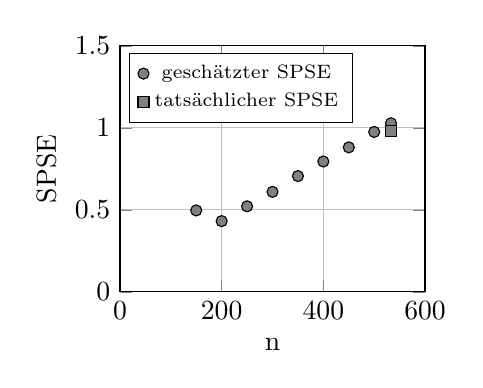
\begin{tikzpicture}
        \begin{axis}[ 
            ylabel = SPSE,
            xlabel = n,
            xmin=0, xmax=600,
            ymin=0, ymax=1.5,
            legend pos = north west,
            scaled ticks = false,
            width = .45\textwidth,
            ymajorgrids,
            xmajorgrids,
            %height = 8cm,
            cycle list name=black white
        ]
            \addplot +[only marks]
            coordinates {
                (150,0.4964226)
                (200,0.4312206)
                (250,0.5213190)
                (300,0.6097658)
                (350,0.7058959)
                (400,0.7947748)
                (450,0.8807918)
                (500,0.9750933)
                (533,1.0280917)
            };
            \addlegendentry{{\scriptsize geschätzter SPSE}}
            
            \addplot +[only marks]
            coordinates {
                (533,0.9813258)
            };
            \addlegendentry{{\scriptsize tatsächlicher SPSE}}
        \end{axis}
    \end{tikzpicture}
    \captionof{figure}{geschätzer sowie tatsächlicher SPSE in Abhängigkeit der Stichprobengröße}
    \label{fig:spse}
\end{figure}

\subsection{Simulation}
\label{ssec:discuss:simulation}
Die vorliegende Arbeit sollte den Einfluss des Stichprobenumfangs auf die SPSE-Schätzung mithilfe Mallow's Cp untersuchen. Die hier angegebenen Werte spiegeln den Mittelwert aus 10 Durchläufen wieder.

\begin{table}[]
	\caption{Über Mallow's Cp geschätzte SPSE Werte mit zugehörigen $n$}
	\begin{tabular}{|l|l|}
		\cline{1-2}
		$n$   & $\hat{SPSE}$ \\ 		\cline{1-2}
		150 &  0.4964226   \\ \cline{1-2}
		200 &  0.4312206   \\ \cline{1-2}
		250 &  0.521319    \\ \cline{1-2}
		300 &  0.6097658  \\ \cline{1-2}
		350 &  0.7058959   \\ \cline{1-2}
		400 &  0.7947748 \\ \cline{1-2}
		450 &  0.8807918  \\ \cline{1-2}
		500 &  0.9750933   \\ \cline{1-2}
		533 &  1.028092   \\ \cline{1-2}

						\end{tabular}
\end{table}

Wie in Abbildung \ref{fig:spse} zu erkennen ist steigt der geschätzte SPSE-Wert außer bei simN < 200 monoton und nahezu linear mit zunehmender Stichprobengröße. Dies lässt auf einen starken linearen Einfluss von $n$ auf den SPSE-Wert schließen. In der Berechnung des SPSE ist $n$ sowohl als Faktor im unkontrollierten Prognosefehler als auch im Biasterm vorhanden, was den Einfluss auf das Ergebnis bereits vermuten ließ.
Der tatsächliche SPSE - Wert von 0,981 wird bei der Schätzung über Mallow's Cp mit derselben Stichprobengröße (533) um 0,048\% überschätzt und liegt bei 1,028. 
Daraus lässt sich schließen, dass der Biasterm durch die zufällige Simulation wohl leicht überschätzt wurde.
Eine Schlussfolgerung aus den hier vorgefundenen Werten ist nun, dass SPSE Werte zur Vergleichbarkeit mittels des Stichprobenumfangs genormt sein müssen, um miteinander vergleichbar zu sein.